\documentclass[12pt, fullpage,letterpaper]{article}

\usepackage[margin=1in]{geometry}
\usepackage{url}
\usepackage{amsmath}
\usepackage{amssymb}
\usepackage{epsfig}
\usepackage{xspace}
\usepackage{graphicx}
\usepackage{hyperref}
\usepackage{xcolor}
\usepackage{ulem}
\usepackage{cancel}
\usepackage{float}

\newcommand\Ccancel[2][black]{\renewcommand\CancelColor{\color{#1}}\cancel{#2}}


\def\red{\color{red}}
\def\blue{\color{blue}}
\def\blackblue{\color{black!40!blue}}

\newcommand{\semester}{Spring 2022}
\newcommand{\assignmentId}{1}
\newcommand{\releaseDate}{1 Feb, 2022}
\newcommand{\dueDate}{11:59pm, 18 Feb, 2022}

\newcommand{\bx}{{\bf x}}
\newcommand{\bw}{{\bf w}}

\title{CS 6190: Probabilistic Machine Learning \semester}
\author{Homework \assignmentId\\
{\red Meysam Alishahi (U1323606)}}
\date{Handed out: \releaseDate\\
  Due: \dueDate}

\begin{document}
\maketitle

% Math commands by Thomas Minka
\newcommand{\var}{{\rm var}}
\newcommand{\Tr}{^{\rm T}}
\newcommand{\vtrans}[2]{{#1}^{(#2)}}
\newcommand{\kron}{\otimes}
\newcommand{\schur}[2]{({#1} | {#2})}
\newcommand{\schurdet}[2]{\left| ({#1} | {#2}) \right|}
\newcommand{\had}{\circ}
\newcommand{\diag}{{\rm diag}}
\newcommand{\invdiag}{\diag^{-1}}
\newcommand{\rank}{{\rm rank}}
% careful: ``null'' is already a latex command
\newcommand{\nullsp}{{\rm null}}
\newcommand{\tr}{{\rm tr}}
\renewcommand{\vec}{{\rm vec}}
\newcommand{\vech}{{\rm vech}}
\renewcommand{\det}[1]{\left| #1 \right|}
\newcommand{\pdet}[1]{\left| #1 \right|_{+}}
\newcommand{\pinv}[1]{#1^{+}}
\newcommand{\erf}{{\rm erf}}
\newcommand{\hypergeom}[2]{{}_{#1}F_{#2}}

% boldface characters
\renewcommand{\a}{{\bf a}}
\renewcommand{\b}{{\bf b}}
\renewcommand{\c}{{\bf c}}
\renewcommand{\d}{{\rm d}}  % for derivatives
\newcommand{\e}{{\bf e}}
\newcommand{\f}{{\bf f}}
\newcommand{\g}{{\bf g}}
\newcommand{\h}{{\bf h}}
%\newcommand{\k}{{\bf k}}
% in Latex2e this must be renewcommand
\renewcommand{\k}{{\bf k}}
\newcommand{\m}{{\bf m}}
\newcommand{\mb}{{\bf m}}
\newcommand{\n}{{\bf n}}
\renewcommand{\o}{{\bf o}}
\newcommand{\p}{{\bf p}}
\newcommand{\q}{{\bf q}}
\renewcommand{\r}{{\bf r}}
\newcommand{\s}{{\bf s}}
\renewcommand{\t}{{\bf t}}
\renewcommand{\u}{{\bf u}}
\renewcommand{\v}{{\bf v}}
\newcommand{\w}{{\bf w}}
\newcommand{\x}{{\bf x}}
\newcommand{\y}{{\bf y}}
\newcommand{\z}{{\bf z}}
%s\newcommand{\l}{\boldsymbol{l}}
\newcommand{\A}{{\bf A}}
\newcommand{\B}{{\bf B}}
\newcommand{\C}{{\bf C}}
\newcommand{\D}{{\bf D}}
\newcommand{\E}{{\bf E}}
\newcommand{\F}{{\bf F}}
\newcommand{\G}{{\bf G}}
\renewcommand{\H}{{\bf H}}
\newcommand{\I}{{\bf I}}
\newcommand{\J}{{\bf J}}
\newcommand{\K}{{\bf K}}
\renewcommand{\L}{{\bf L}}
\newcommand{\M}{{\bf M}}
\newcommand{\N}{\mathcal{N}}  % for normal density
\newcommand{\Dcal}{\mathcal{D}}  % for normal density

%\newcommand{\N}{{\bf N}}
\renewcommand{\O}{{\bf O}}
\renewcommand{\P}{{\bf P}}
\newcommand{\Q}{{\bf Q}}
\newcommand{\R}{{\bf R}}
\renewcommand{\S}{{\bf S}}
\newcommand{\T}{{\bf T}}
\newcommand{\U}{{\bf U}}
\newcommand{\V}{{\bf V}}
\newcommand{\W}{{\bf W}}
\newcommand{\X}{{\bf X}}
\newcommand{\Y}{{\bf Y}}
\newcommand{\Z}{{\bf Z}}

% this is for latex 2.09
% unfortunately, the result is slanted - use Latex2e instead
%\newcommand{\bfLambda}{\mbox{\boldmath$\Lambda$}}
% this is for Latex2e
\newcommand{\bfLambda}{\boldsymbol{\Lambda}}

% Yuan Qi's boldsymbol
\newcommand{\bsigma}{\boldsymbol{\sigma}}
\newcommand{\balpha}{\boldsymbol{\alpha}}
\newcommand{\bpsi}{\boldsymbol{\psi}}
\newcommand{\bphi}{\boldsymbol{\phi}}
\newcommand{\boldeta}{\boldsymbol{\eta}}
\newcommand{\Beta}{\boldsymbol{\eta}}
\newcommand{\btau}{\boldsymbol{\tau}}
\newcommand{\bvarphi}{\boldsymbol{\varphi}}
\newcommand{\bzeta}{\boldsymbol{\zeta}}

\newcommand{\blambda}{\boldsymbol{\lambda}}
\newcommand{\bLambda}{\mathbf{\Lambda}}
\newcommand{\bOmega}{\mathbf{\Omega}}
\newcommand{\bomega}{\mathbf{\omega}}
\newcommand{\bPi}{\mathbf{\Pi}}

\newcommand{\btheta}{\boldsymbol{\theta}}
\newcommand{\bpi}{\boldsymbol{\pi}}
\newcommand{\bxi}{\boldsymbol{\xi}}
\newcommand{\bSigma}{\boldsymbol{\Sigma}}

\newcommand{\bgamma}{\boldsymbol{\gamma}}
\newcommand{\bGamma}{\mathbf{\Gamma}}

\newcommand{\bmu}{\boldsymbol{\mu}}
\newcommand{\1}{{\bf 1}}
\newcommand{\0}{{\bf 0}}

% \newcommand{\comment}[1]{}

\newcommand{\bs}{\backslash}
\newcommand{\ben}{\begin{enumerate}}
\newcommand{\een}{\end{enumerate}}

 \newcommand{\notS}{{\backslash S}}
 \newcommand{\nots}{{\backslash s}}
 \newcommand{\noti}{{\backslash i}}
 \newcommand{\notj}{{\backslash j}}
 \newcommand{\nott}{\backslash t}
 \newcommand{\notone}{{\backslash 1}}
 \newcommand{\nottp}{\backslash t+1}
% \newcommand{\notz}{\backslash z}

\newcommand{\notk}{{^{\backslash k}}}
%\newcommand{\noti}{{^{\backslash i}}}
\newcommand{\notij}{{^{\backslash i,j}}}
\newcommand{\notg}{{^{\backslash g}}}
\newcommand{\wnoti}{{_{\w}^{\backslash i}}}
\newcommand{\wnotg}{{_{\w}^{\backslash g}}}
\newcommand{\vnotij}{{_{\v}^{\backslash i,j}}}
\newcommand{\vnotg}{{_{\v}^{\backslash g}}}
\newcommand{\half}{\frac{1}{2}}
\newcommand{\msgb}{m_{t \leftarrow t+1}}
\newcommand{\msgf}{m_{t \rightarrow t+1}}
\newcommand{\msgfp}{m_{t-1 \rightarrow t}}

\newcommand{\proj}[1]{{\rm proj}\negmedspace\left[#1\right]}
\newcommand{\argmin}{\operatornamewithlimits{argmin}}
\newcommand{\argmax}{\operatornamewithlimits{argmax}}

\newcommand{\dif}{\mathrm{d}}
\newcommand{\abs}[1]{\lvert#1\rvert}
\newcommand{\norm}[1]{\lVert#1\rVert}

%miscellaneous symbols
\newcommand{\ie}{{{i.e.,}}\xspace}
\newcommand{\eg}{{{\em e.g.,}}\xspace}
\newcommand{\EE}{\mathbb{E}}
\newcommand{\VV}{\mathbb{V}}
\newcommand{\sbr}[1]{\left[#1\right]}
\newcommand{\rbr}[1]{\left(#1\right)}
\newcommand{\cmt}[1]{}



\footnotesize

\section*{Analytical problems [80 points + 30 bonus]}	
\label{sec:q1}

\begin{enumerate}
\item~[8 points] A random vector, $\x = \left[\begin{array}{c}\x_1 \\  \x_2\end{array}\right]$ follows a multivariate Gaussian distribution, 
\[
p(\x) = \N\big( \left[\begin{array}{c}\x_1 \\  \x_2\end{array}\right] |  \left[\begin{array}{c}\bmu_1 \\  \bmu_2\end{array}\right], \left[\begin{array}{cc} \bSigma_{11} & \bSigma_{12} \\  \bSigma_{21} & \bSigma_{22}\end{array}\right]\big).
\]
Show that the marginal distribution of $\x_1$ is $p(\x_1) = \N(\x_1| \bmu_1, \bSigma_{11})$.\\
{\red Answer: }{\blackblue 
Set $\bSigma = \left[\begin{array}{cc} \bSigma_{11} & \bSigma_{12} \\  \bSigma_{21} & \bSigma_{22}\end{array}\right]$ and 
$\bSigma^{-1} = \bLambda = \left[\begin{array}{cc} \bLambda_{11} & \bLambda_{12} \\  \bLambda_{21} & \bLambda_{22}\end{array}\right]$. 
  In the class, it was proved that 
$$p(\x_2|\x_1) = \N\big(\x_2|\bmu_{2|1},\bSigma_{2|1}\big),$$
where $\bSigma_{2|1} = \bLambda^{-1}_{22}$ and $\bmu_{2|1}=\bmu_2 - \bLambda_{22}^{-1}\bLambda_{21}(x_1-\bmu_1)$.
Using Bayes' Rule,  
\begin{equation}\label{CQ1}
p(\x_1) = \frac{p(\x_1,\x_2)}{p(\x_2|\x_1)}= C\exp\left\{-\frac12 (A-B)\right\},
\end{equation}
where $C$ is a constant with respect to $\x_1$ and $\x_2$, 
 $$A = \left[(\x_1-\bmu_1)^\top,(\x_2-\bmu_2)^\top\right] \left[\begin{array}{cc} \bLambda_{11} & \bLambda_{12} \\  \bLambda_{21} & \bLambda_{22}\end{array}\right]
\left[\begin{array}{c}\x_1-\bmu_1 \\  \x_2 -\bmu_2 \end{array}\right]$$
and 
$B = (\x_2-\bmu_{2|1})^\top\bSigma_{2|1}^{-1}(\x_2-\bmu_{2|1}).$
So, to know $p(\x_1)$, we need to compute $A-B$. Expanding $A$, we have 
\begin{align*}
A = & (\x_1-\bmu_1)^\top \bLambda_{11}(\x_1-\bmu_1) + (\x_1-\bmu_1)^\top \bLambda_{12}(\x_2 -\bmu_2) \\
& + (\x_2-\bmu_2)^\top \bLambda_{21}(\x_1-\bmu_1) + (\x_2-\bmu_2)^\top \bLambda_{22}(\x_2 -\bmu_2).
\end{align*}
We saw in the class that 
$p(\x_2|\x_1) = \N\big(x_2|\bmu_{2|1},\bSigma_{2|1}\big),$
where $\bSigma_{2|1} = \bLambda^{-1}_{22}$ and $\bmu_{2|1}=\bmu_2 - \bLambda_{22}^{-1}\bLambda_{21}(x_1-\bmu_1)$.
Also, expanding $B$ and also using the facts that $\bSigma_{2|1} = \bLambda^{-1}_{22}$ and $\bmu_{2|1}=\bmu_2 - \bLambda_{22}^{-1}\bLambda_{21}(x_1-\bmu_1)$, we conclude 
\begin{align*}
B & = (\x_2-\bmu_{2|1})^\top\bSigma_{2|1}^{-1}(\x_2-\bmu_{2|1})\\
& = \Big(\x_2-\bmu_2 + \bLambda_{22}^{-1}\bLambda_{21}(x_1-\bmu_1)\Big)^\top \bLambda_{22}\Big(\x_2-\bmu_2 + \bLambda_{22}^{-1}\bLambda_{21}(x_1-\bmu_1)\Big)\\ 
& = (\x_2-\bmu_2)^\top\bLambda_{22}(\x_2-\bmu_2) \\ 
& + (\x_2-\bmu_2)^\top\bLambda_{22}\bLambda_{22}^{-1}\bLambda_{21}(x_1-\bmu_1)\\
& + (x_1-\bmu_1)^\top\bLambda_{21}^\top\bLambda_{22}^{-1}\bLambda_{22}(\x_2-\bmu_2) \\
& + (x_1-\bmu_1)^\top\bLambda_{21}^\top\bLambda_{22}^{-1} \bLambda_{22}\bLambda_{22}^{-1}\bLambda_{21}(x_1-\bmu_1)\\
& = (\x_2-\bmu_2)^\top\bLambda_{22}(\x_2-\bmu_2) + (\x_2-\bmu_2)^\top\bLambda_{21}(x_1-\bmu_1)\\
& + (x_1-\bmu_1)^\top\bLambda_{21}^\top(\x_2-\bmu_2) + (x_1-\bmu_1)^\top\bLambda_{21}^\top\bLambda_{22}^{-1}\bLambda_{21}(x_1-\bmu_1)
\end{align*}
Therefore, 
\begin{align*}
A - B 
& = (\x_1-\bmu_1)^\top \underbrace{\left(\bLambda_{11}- \bLambda_{21}^\top\bLambda_{22}^{-1}\bLambda_{21}\right)}_{=\bSigma_{11}^{-1}}(x_1-\bmu_1)\\
& = (\x_1-\bmu_1)^\top\bSigma_{11}^{-1} (\x_1-\bmu_1)
\end{align*}
Substituting in \ref{CQ1}, 
$$p(\x_1) = C\exp\left\{-\frac12 \Big((\x_1-\bmu_1)^\top\bSigma_{11}^{-1} (\x_1-\bmu_1)\Big)\right\}.$$
Since $p(\x_1)$ is a pdf, $C$ should be $|2\pi\Sigma_{11}|^{-1}$ and consequently, 
$p(\x_1) = \N(\x_1| \bmu_1, \bSigma_{11})$ as desired. 
}
\item~[\textbf{Bonus}][10 points] Given a Gaussian random vector, $\x \sim \N(\x|\bmu, \bSigma)$.  We have a linear transformation, $\y = \A\x + \b + \z$, where $\A$ and $\b$ are constants, $\z$ is another Gaussian random vector independent to $\x$, $p(\z) = \N(\z|\0, \bLambda)$. Show $\y$ follows Gaussian distribution as well, and derive its form. Hint: using characteristic function. You need to check the materials by yourself. \\
{\red Answer: }{\blackblue  
First note that since since $\x$ and $\z$ are independent,  $\x' = \A\x + \b$ and $\z$ are independent as well. 
We remind that the characteristic function of a random variable $\x$ with probability distribution function $p(\x)$ is defined as
$$\phi_\x(\t) = \EE_p(e^{i\t^\top\x}).$$
Also, it is a known fact that $\x\sim \N(\bmu, \bSigma)$ if and only if $\phi_\x(\t) = e^{\t^\top(i\bmu - \frac{1}{2}\bSigma\t)}$.
Let us compute $\phi_\y(\t)$.
\begin{align*}
\phi_\y(\t) & =  \EE_y(e^{i\t^\top\y})=  \EE_\y\left(e^{i\t^\top(\A\x + \b + \z)}\right)\\
 & =  e^{i\t^\top\b}\EE_\x\left(e^{i\t^\top\A\x }\right)\EE_\z\left(e^{i\t^\top \z}\right)\qquad \mbox{since $\A\x$ and $\z$ are independent and $\b$ is constant} \\
& = e^{i\t^\top\b}  e^{\t^\top(i\A\bmu - \frac{1}{2}\A\bSigma \A^\top\t)}   e^{\t^\top(- \frac{1}{2}\bLambda\t)} \qquad
\mbox{ since $\A\x \sim \N(\A\bmu, \A\bSigma\A^\top)$ and $\z\sim \N(0,\bLambda)$}\\
& = e^{\t^\top\Big(i(\A\bmu + \b) -\frac12 (\A\bSigma\A^\top+\bLambda)\t \Big)}.
\end{align*} 
Therefore, $\y \sim \N(\A\bmu + \b, \A\bSigma\A^\top+\bLambda).$
}
\item~[8 points] Show the differential entropy of the a multivariate Gaussian distribution $\N(\x|\bmu, \bSigma)$ is
\[
\mathrm{H}[\x] = \frac{1}{2}\log |\bSigma| + \frac{d}{2}(1 + \log 2\pi)
\]
where $d$ is the dimension of $\x$.
{\red Answer: }{\blackblue  
If $\x \sim \N(\x|\bmu, \bSigma)$, then $f(\x) = (2\pi)^{-d/2}|\bSigma|^{-1/2}e^{-\frac{1}{2}(\x-\bmu)^\top\bSigma^{-1}(\x-\bmu)}$.
Accordingly,
\begin{align*}
H[\x] &= -\int_{x\in \mathbb{R}^d} f(\x)\log f(\x) \d \x = -\int_{x\in \mathbb{R}^d} f(\x)\left[-\frac{d}{2}\log 2\pi -\frac12\log|\bSigma| -\frac{1}{2}(\x-\bmu)^\top\bSigma^{-1}(\x-\bmu)\right] \d \x \\
& = \int_{x\in \mathbb{R}^d} f(\x)\left[\frac{d}{2}\log 2\pi +\frac12\log|\bSigma| +\frac{1}{2}(\x-\bmu)^\top\bSigma^{-1}(\x-\bmu)\right] \d \x \\
& = \frac{d}{2}\log 2\pi \underbrace{\int_{x\in \mathbb{R}^d} f(\x)\d\x}_\text{$=1$ because $f$ is a pdf} +\frac12\log|\bSigma| \underbrace{\int_{x\in \mathbb{R}^d} f(\x)\d\x}_\text{$=1$ because $f$ is a pdf} + \frac{1}{2}\int_{x\in \mathbb{R}^d} f(\x)(\x-\bmu)^\top\bSigma^{-1}(\x-\bmu) \d \x \\
& = \frac{d}{2}\log 2\pi +\frac12\log|\bSigma| + \frac{1}{2}\EE_{\x \sim \N(\x|\bmu, \bSigma)}\Big[(\x-\bmu)^\top\bSigma^{-1}(\x-\bmu)\Big] \\
& = \frac{d}{2}\log 2\pi +\frac12\log|\bSigma| + \frac{1}{2}\EE_{\x \sim \N(\x|\bmu, \bSigma)}\Big[\tr \left((\x-\bmu)^\top\bSigma^{-1}(\x-\bmu)\right)\Big] \\
& = \frac{d}{2}\log 2\pi +\frac12\log|\bSigma| + \frac{1}{2}\EE_{\x \sim \N(\x|\bmu, \bSigma)}\Big[\tr \left((\x-\bmu)(\x-\bmu)^\top\bSigma^{-1}\right)\Big] \\
& = \frac{d}{2}\log 2\pi +\frac12\log|\bSigma| + \frac{1}{2}\tr \left(\underbrace{\EE_{\x \sim \N(\x|\bmu, \bSigma)}\Big[(\x-\bmu)(\x-\bmu)^\top\Big]}_\text{\red $=\bSigma$}\bSigma^{-1}\right) \\
& = \frac{d}{2}\log 2\pi +\frac12\log|\bSigma| + \frac{1}{2}\tr \left(\I_{d\times d}\right) 
 = \frac{d}{2}\log 2\pi +\frac12\log|\bSigma| + \frac{d}{2}.
\end{align*}}
\vspace{-.5cm}
\item~[8 points] Derive the Kullback-Leibler divergence between two Gaussian distributions, $p(\x) = \N(\x|\bmu, \bSigma)$ and $q(\x) = \N(\x|\m, \Lambda)$, \ie $\mathrm{KL}(q || p)$.
{\red Answer: }{\blackblue Lets remind that 
\begin{align*}
\mathrm{KL}(q || p) 
& = \int_{x\in\mathbb{R}^d} q(\x)\log\frac{q(\x)}{p(\x)}\d\x = \underbrace{\int_{x\in\mathbb{R}^d} q(\x)\log q(\x)\d\x}_\text{$= -H_p[\x]$, See question 3.} - \underbrace{\int_{x\in\mathbb{R}^d} q(\x)\log p(\x) \d\x}_\text{is computed in the following}\\
& = - \frac{1}{2}\log |\bLambda| - \frac{d}{2}(1 + \log 2\pi) +
(\frac{d}{2}\log 2\pi +\frac12\log|\bSigma|) +\frac12\tr\left( \Big[\Lambda +\m\m^\top -\m\bmu^\top  - \bmu\m^\top + \bmu\bmu^\top\Big]\bSigma^{-1}\right)\\
& = \frac{1}{2}\log |\bSigma| - \frac{d}{2} - \frac12\log|\Lambda| +\frac12\tr\left( \Big[\Lambda +\m\m^\top -\m\bmu^\top  - \bmu\m^\top + \bmu\bmu^\top\Big]\bSigma^{-1}\right).\\
& = \frac{1}{2}\log \frac{|\bSigma|}{|\Lambda|} - \frac{d}{2}  +
\frac12\left(\tr(\Lambda\bSigma^{-1}) + \m^\top\bSigma^{-1}\m - 2\bmu^\top\bSigma^{-1}\m  +  \bmu^\top\bSigma^{-1} \bmu\right)
\end{align*}
So, we need to compute  $\int_{x\in\mathbb{R}^d} q(\x)\log p(\x) \d\x$. 
\begin{align*}
\int_{x\in \mathbb{R}^d} q(\x)\log p(\x) \d \x 
& = -\int_{x\in \mathbb{R}^d} q(\x)\left[\frac{d}{2}\log 2\pi +\frac12\log|\bSigma| +\frac{1}{2}(\x-\bmu)^\top\bSigma^{-1}(\x-\bmu)\right] \d \x \\
& = -(\frac{d}{2}\log 2\pi +\frac12\log|\bSigma|)\underbrace{\int_{x\in \mathbb{R}^d} q(\x)\d\x}_\text{$=1$} -\frac{1}{2}\underbrace{\int_{x\in \mathbb{R}^d} q(\x)(\x-\bmu)^\top\Lambda^{-1}(\x-\bmu)\d \x}_\text{$=\EE_q\Big[(\x-\bmu)^\top\bSigma^{-1}(\x-\bmu)\Big]$}  \\
& = -(\frac{d}{2}\log 2\pi +\frac12\log|\bSigma|) -\frac12 \EE_q\Big[\tr\left((\x-\bmu)^\top\bSigma^{-1}(\x-\bmu)\right)\Big]\\
& = -(\frac{d}{2}\log 2\pi +\frac12\log|\bSigma|) -\frac12 \EE_q\Big[\tr\left((\x-\bmu)(\x-\bmu)^\top\bSigma^{-1}\right)\Big]\\
& = -(\frac{d}{2}\log 2\pi +\frac12\log|\bSigma|) -\frac12\tr\left( \EE_q\Big[(\x-\bmu)(\x-\bmu)^\top\Big]\bSigma^{-1}\right)\\
& = -(\frac{d}{2}\log 2\pi +\frac12\log|\bSigma|) -\frac12\tr\left( \EE_q\Big[\x\x^\top - \x\bmu^\top-\bmu\x^\top +\bmu\bmu^\top\Big]\bSigma^{-1}\right)\\
& = -(\frac{d}{2}\log 2\pi +\frac12\log|\bSigma|) -\frac12\tr\left( \Big[\Lambda +\m\m^\top -\m\bmu^\top  - \bmu\m^\top + \bmu\bmu^\top\Big]\bSigma^{-1}\right)
\end{align*}
}

\item~[8 points] Given a distribution in the exponential family, 
\[
p(\x|\boldeta) = \frac{1}{Z(\boldeta)} h(\x)\exp\big(-\u(\x)^\top \boldeta\big).
\]
Show that 
\[
\frac{\partial^2 \log Z(\boldeta)}{\partial \boldeta^2} = \mathrm{cov}(\u(\x)), 
\]
where $\mathrm{cov}$ is the covariance matrix. 
{\red Answer: }{\blackblue 
Notice 
$Z(\boldeta) = \int h(\x)\exp\big(-\u(\x)^\top \boldeta\big)\d\x.$
Consequently, 
\begin{align*}
\frac{\partial \log Z(\boldeta)}{\partial \boldeta}  
& = \frac{1}{Z(\boldeta) }\frac{\partial Z(\boldeta)}{\partial \boldeta}  = \frac{1}{Z(\boldeta) }\frac{\partial }{\partial \boldeta} \int h(\x)\exp\big(-\u(\x)^\top \boldeta\big)\d\x  \\
& = \frac{1}{Z(\boldeta)}  \int \frac{\partial }{\partial \boldeta}\Big(h(\x)\exp\big(-\u(\x)^\top \boldeta\big)\Big)\d\x = -\frac{1}{Z(\boldeta)}  \int h(\x)\exp\big(-\u(\x)^\top \boldeta\big)\u(\x)\d\x\\
& = -\int\underbrace{\frac{1}{Z(\boldeta)}   h(\x)\exp\big(-\u(\x)^\top \boldeta\big)}_{=p(\x|\boldeta)}\u(\x)\d\x = -\EE(\u(\x)).
\end{align*}
Therefore, 
\begin{align*}
\frac{\partial^2 \log Z(\boldeta)}{\partial \boldeta^2}
%& = -\frac{\partial }{\partial \boldeta}\left(\frac{1}{Z(\boldeta)}  \int h(\x)\exp\big(-\u(\x)^\top \boldeta\big)\u(\x)\d\x\right)^\top\\
& = -\frac{\partial }{\partial \boldeta}
\left(\frac{1}{Z(\boldeta)}  \int h(\x)\exp\big(-\u(\x)^\top \boldeta\big)\u(\x)^\top\d\x\right)\\ \\
& = -\frac{1}{Z(\boldeta)^2}\underbrace{\frac{\partial Z(\boldeta)}{\partial \boldeta}}_{= \int h(\x)\exp\big(-\u(\x)^\top \boldeta\big)\u(\x)\d\x}
\int h(\x)\exp\big(-\u(\x)^\top \boldeta\big)\u(\x)^\top\d\x \\
& +  \frac{1}{Z(\boldeta)}  \int \frac{\partial }{\partial \boldeta}\Big(h(\x)\exp\big(-\u(\x)^\top \boldeta\big)\u(\x)\Big)\d\x\\ \\
 & = -\left[\int \frac{1}{Z(\boldeta)}h(\x)\exp\big(-\u(\x)^\top \boldeta\big)\u(\x)\d\x\right]\left[\int \frac{1}{Z(\boldeta)}h(\x)\exp\big(-\u(\x)^\top \boldeta\big)\u(\x)^\top\d\x\right] \\
& +  \int \frac{1}{Z(\boldeta)}  h(\x)\exp\big(-\u(\x)^\top \boldeta\big)\u(\x)\u(\x)^\top\d\x \\
& = -\left[\int p(\x|\boldeta)\u(\x)\d\x\right]\left[\int p(\x|\boldeta)\u(\x)^\top\d\x\right] 
+  \int p(\x|\boldeta)\u(\x)\u(\x)^\top\d\x \\
 & = -\EE(\u(\x))\EE(\u(\x))^\top + \EE(\u(\x)\u(\x)^\top) = \mathrm{cov}(\u(\x))
\end{align*}}
\vspace{-.5cm}
\item~[4 points] Is $\log Z(\boldeta)$ convex or nonconvex? Why?
{\red Answer: }{\blackblue It is convex since the covariance matrix of any random variable is positive semi-definite.\\
{\bf Observation.} {\it If $\z$ is a random variable, then  $\mathrm{cov}(\z)$ is positive semi-definite.}\\
{\bf Proof.} Let $\y$ be an arbitrary vector, we need to prove that $\y^t\mathrm{cov}(\z)\y\geq 0$. 
To this end;
\begin{align*}
\y^t\mathrm{cov}(\z)\y & = \y^t\EE\big(\z\z^\top\big)\y = \EE\big(\y^\top\z\z^\top\y)\\
& = \EE\left[\big(\z^\top\y)(\z^\top\y)\right] = \EE\left[\big(\z^\top\y)^2\right]\geq 0, 
\end{align*}
since $(\z^\top\y)^2\geq 0$ and expectation of any nonnegative random variable is nonnegative. 
} 

\item~[8 points] Given two random variables $\x$ and $\y$, show that
\[
I(\x,\y) = H[\x] - H[\x|\y]
\]
where $I(\cdot, \cdot)$ is the mutual information and $H[\cdot]$ the entropy.\\
{\red Answer: }{\blackblue 
\begin{align*}
\I[\x,\y]  & = {\rm KL}\Big(p(\x,\y)|| p(\x)p(\y)\Big)
 = -\int\int p(\x,\y)\ln\left(\frac{p(\x)p(\y)}{p(\x,\y)}\right)\d\x\d\y\\
& = -\int\int p(\x,\y)\ln\left(\frac{p(\x)\Ccancel[red]{p(\y)}}{p(\x|\y)\Ccancel[red]{p(\y)}}\right)\d\x\d\y 
= -\int\int p(\x,\y)\ln p(\x)\d\x\d\y + \underbrace{\int\int p(\x,\y)\ln p(\x|\y)\d\x\d\y}_{=-H[\x|\y]} \\
& = -\int\underbrace{\Big[\int p(\x,\y)\d\y\Big]}_{=p(\x)}\ln p(\y)\d\x - H[\x|\y] = \underbrace{-\int p(\x)\ln p(\x)\d\x}_{=H[\x]} - H[\x|\y] = H[\x] - H[\x|\y].
\end{align*}
}

\item~[24 points] Convert the following distributions into the form of the exponential-family distribution. Please give the mapping from the expectation parameters to the natural parameters, and also represent the log normalizer as a function of the natural parameters.
\begin{itemize}
	\item Dirichlet distribution
	\item Gamma distribution
	\item Wishart distribution
\end{itemize}
{\red Answer: }{\blackblue 
Any distribution can be written as the following form is a member of exponential family;
\[
p(\x|\boldeta) = \frac{1}{Z(\boldeta)} h(\x)\exp\big(-\u(\x)^\top \boldeta\big).
\]
{\red \bf Dirichlet distribution.} Let us remind that for $\balpha = (\alpha_1,\cdots,\alpha_d)$,  and $\alpha_0 = \sum_{i=1}^d\alpha_i$, Dirichlet distribution ${\rm Dir}(\x|\balpha)$ is a probability density function over $(d-1)$-simplex (i.e.,  $\x=(x_1,\ldots,\x_d)\in \Delta_{d-1}$) with the following density function;   
\begin{align*}
{\rm Dir}(\x|\balpha) 
& = \underbrace{\frac{\Gamma(\alpha_0)}{\Gamma(\alpha_1)\cdots\Gamma(\alpha_d)}}_{=C(\balpha)}\prod_{i=1}^dx_i^{\alpha_k-1}
 = C(\balpha) \exp\left(\sum_{i=1}^d (\alpha_i-1)\ln x_i\right) \\
& = C(\balpha) \frac{1}{\prod_{i=1}^dx_i}\exp\left(\sum_{i=1}^d \alpha_i\ln x_i\right)  
= \frac{1}{Z(\boldeta)}h(\x) \exp\left(-\u(\x)^\top\boldeta\right),
\end{align*}
where $$h(\x) = \frac{1}{\prod_{i=1}^dx_i}, \quad\quad\quad \boldeta =(\alpha_1,\ldots, \alpha_d)^\top,$$
$$\u(\x) = (-\ln x_1,\ldots,-\ln x_d)^\top, \quad\quad\quad Z(\boldeta)= \frac{\Gamma\left(\sum_{i=1}^d\boldeta_i\right)}{\Gamma(\boldeta_1)\cdots\Gamma(\boldeta_d)}.$$ 

{\red \bf Gamma distribution.}
\begin{align*}
{\rm Gam}(x|a,b) 
& = \frac{1}{\Gamma(a)}b^ax^{a-1}\exp(-bx) \quad\quad\mbox{where  $a>0, b>0$}\\
& = \frac{1}{\Gamma(a)}b^ax^{-1}\exp(-bx + a\ln x)  = \frac{1}{\Gamma(a)b^{-a}}\frac{1}{x}\exp(-[a,b][-\ln x,x]^\top) \\
& = \frac{1}{Z(\boldeta)}h(x) \exp\left(-\u(x)^\top\boldeta\right),
\end{align*}
where $\quad\quad\quad h(x) = \frac{1}{x}, \quad\quad\boldeta = [a,b],\quad\quad \u(x) = [-\ln x,x], \quad\quad Z(\boldeta) = \Gamma(a)b^{-a} = \Gamma(\boldeta_1)\boldeta_2^{-\boldeta_1}.$


{\red \bf Wishart distribution.}
Let $\X$ be a $d\times d$ symmetric matrix of random variables that is positive definite.  If $\nu\geq d$, we say $\X$ has a Wishart distribution with $\nu$ degrees of freedom if it has the probability density function
$$\bomega(\X|\W,\nu) = \frac{|\X|^{\frac{\nu-d-1}{2}}\exp\left(-\frac12\tr\left(\W^{-1}\X\right)\right)}{2^{\frac{d\nu}{2}}|\W|^{\frac{\nu}{2}}\Gamma_d(\frac{\nu}{2})},$$
where $\Gamma_d(\cdot)$ is the multivariate gamma function.
\begin{align*}
\bomega(\X|\W,\nu) 
& = \frac{|\X|^{\frac{\nu-d-1}{2}}\exp\left(-\frac12\tr\left(\W^{-1}\X\right)\right)}{2^{\frac{d\nu}{2}|\W|^{\frac{\nu}{2}}\Gamma_d(\frac{\nu}{2})}}\\
& = \frac{|\X|^\frac{-d-1}{2}\exp\left(\frac{\nu}{2}\ln |\X|-\frac12\tr\left(\W^{-1}\X\right)\right)}{2^{\frac{d\nu}{2}}|\W|^{\frac{\nu}{2}\Gamma_d(\frac{\nu}{2})}}\\
& = \frac{1}{2^{\frac{d\nu}{2}}|\W|^{\frac{\nu}{2}\Gamma_d(\frac{\nu}{2})}}
|\X|^\frac{-d-1}{2}
\exp\left\{-\left(\frac12\vec(\X), -\frac12\ln|\X|\right)\left(\vec(\W^{-1}), \nu\right)^\top\right\}\\
& = \frac{1}{Z(\boldeta)}h(\X) \exp\left(-\u(\X)^\top\boldeta\right),
\end{align*}
where 
$$h(\X)=|\X|^\frac{-d-1}{2}\quad\quad\quad Z(\boldeta) = 2^{\frac{d\nu}{2}}|\W|^{\frac{\nu}{2}}\Gamma_d(\frac{\nu}{2})$$
$$\boldeta  = \left(\vec(\W^{-1}), \nu\right)^\top, \quad\quad\quad \u(\X) = \left(\frac12\vec(\X), -\frac12\ln|\X|\right)^\top.$$


}
\item~[6 points] Does student $t$ distribution (including both the scalar and vector cases) belong to the exponential family? Why?\\
{\red \bf Answer.}{\blackblue 
The student $t$ distribution is given as $f(x) = c(v)(\nu+x^2)^{-\frac{\nu+1}{2}}$.
If we were able to write it as an exponential family, then  
$$c(v)\exp\left({{-\frac{\nu+1}{2}}\ln(\nu+x^2)}\right) = c(v)\exp\left(-\eta(\nu)\u(x)\right)$$
which implies $\eta(\nu)\u(x) = \frac{\nu+1}{2}\ln(\nu+x^2).$ Setting $\nu =1$, we have $u(x) = c \ln(1+x^2)$ where $c= 1/\eta(1)$.
Plugging  $u(x)$ in the above formula, we get  
$$\eta(\nu) = { \frac{\nu+1}{2}\ln(\nu+x^2)\over c \ln(1+x^2)}$$ which is a function of $x$, a contradiction. 
}

\item~[6 points] Does the mixture of Gaussian distribution belong to the exponential family? Why? 
\[
p(\x) = \frac{1}{2}\N(\x|\bmu, \bSigma) + \frac{1}{2}\N(\x|\m, \bLambda)
\]
{\red \bf Answer.} {\blackblue We know that it is impossible to write $\alpha e^x + \beta e^y$ as $c^{f(x,y)}$ if $\alpha\neq \beta$. Therefore, the mixture of Gaussian distribution with different parameters cannot belong to the exponential family.}

\item~[\textbf{Bonus}][20 points] Given a distribution in the exponential family $p(\x|\boldeta)$, where $\boldeta$ are the natural parameters. As we discussed in the class, the distributions in the exponential family are often parameterized by their expectations, namely $\btheta = \EE\big(\u(\x)\big)$ where $\u(\x)$ are the sufficient statistics (recall Gaussian and Bernoulli distributions). Given an arbitrary distribution $p(\x|\balpha)$, the Fisher information matrix in terms of the distribution parameters $\balpha$ is defined as $\F(\balpha) = \EE_{p(\x|\balpha)}[- \frac{\partial^2 \log(p(\x|\balpha)) }{\partial \balpha^2}]$. 
\begin{enumerate}
	\item~[5 points] Show that if we calculate the Fisher Information matrix in terms of the natural parameters, we have $\F(\boldeta) = \mathrm{cov}\big(\u(\x)\big)$.\\
	{\red Answer: }{\blackblue 
	To compute 
	$\F(\boldeta) = \EE_{p(\x|\boldeta)}[- \frac{\partial^2 \log(p(\x|\boldeta)) }{\partial \balpha^2}]$, we first focus on computing 
	$\frac{\partial^2 \log(p(\x|\boldeta)) }{\partial \balpha^2}.$
	\begin{align*}
	\frac{\partial \log(p(\x|\boldeta)) }{\partial \boldeta} 
	& = \frac{\partial \log(p(\x|\boldeta)) }{\partial \boldeta} \\
	& = \frac{\partial }{\partial \boldeta} \log\left[\frac{1}{Z(\boldeta)} h(\x)\exp\big(-\u(\x)^\top \boldeta\big)\right]\\
	& = \frac{\partial }{\partial \boldeta} \left[-\log Z(\boldeta) + \log h(\x) -\u(\x)^\top \boldeta\right]\\
	& = -\frac{\partial \log Z(\boldeta)}{\partial \boldeta}  - \u(\x)
	\end{align*}
	Consequently, using the result proved in Question 
	\begin{align*}
	\frac{\partial^2 \log(p(\x|\boldeta)) }{\partial \boldeta^2}
	& = - \frac{\partial^2 \log Z(\boldeta)}{\partial \boldeta^2}  - \frac{\partial\u(\x)}{\partial \boldeta}\\
	& = -{\rm cov}(\u(x)) + 0 \quad\quad\mbox{using Question 5}\\
	& = -{\rm cov}_{p(\x|\boldeta)}(\u(x))
	\end{align*}
	Finally, since ${\rm cov}_{p(\x|\balpha)}(\u(x))$ is a constant with respect to $\x$, we conclude that 
	\begin{align*}
	\F(\boldeta) & = 
	\EE_{p(\x|\balpha)}\left[- \frac{\partial^2 \log(p(\x|\balpha)) }{\partial \balpha^2}\right] \\
	&= \EE_{p(\x|\balpha)}\left[{\rm cov}(\u(x))\right]
	 = {\rm cov}(\u(x)). 
	\end{align*}
	}
	
	\item~[5 points] Show that $\frac{\partial \btheta}{\partial \boldeta} = \F(\boldeta)$. 
	{\red Answer: }{\blackblue 
	In Question 5, we proved that 
	\begin{align*}
	\btheta 
	 =  \EE(\u(\x))
	 =\frac{\partial \log Z(\boldeta)}{\partial \boldeta}.
	\end{align*}
	Therefore, 
	\begin{align*}
	\frac{\partial \btheta}{\partial \boldeta}  
	& = \frac{\partial^2 \log Z(\boldeta)}{\partial \boldeta^2}\\ 
	& = \mathrm{cov}(\u(\x)) \quad\quad\mbox{proved in Question 5}\\
	& = \F(\boldeta) \quad\quad\mbox{proved in previous section.}
	\end{align*}
	}
	\item~[10 points] Show that the Fisher information matrix in terms of the expectation parameters is the inverse of that in terms of the natural parameters, $\F(\btheta) =\F^{-1}(\boldeta)$.\\
	{\red Answer: }{\blackblue 
	According to the definition, 
	\begin{align*}
	\F(\btheta) & = \EE_{p(\x|\btheta)}[- \frac{\partial^2 \log(p(\x|\btheta)) }{\partial \btheta^2}].
	\end{align*}
	So, we need to compute $\frac{\partial^2 \log(p(\x|\btheta)) }{\partial \btheta^2}$.
	\begin{align*}
	\frac{\partial \log(p(\x|\boldeta)) }{\partial \boldeta} 
	& = \frac{\partial \log(p(\x|\btheta)) }{\partial \btheta} \frac{\partial \btheta}{\partial \boldeta}\\
	& =  \frac{\partial \log(p(\x|\btheta)) }{\partial \btheta} \F(\boldeta)\quad\quad\mbox{from previous part, $\frac{\partial \btheta}{\partial \boldeta}=\F(\boldeta)$}
	\end{align*}
	Consequently, 
	\begin{align*}
	\frac{\partial^2 \log(p(\x|\boldeta)) }{\partial \boldeta^2} 
	 & = \frac{\partial}{\partial \boldeta}\left[\frac{\partial \log(p(\x|\boldeta)) }{\partial \boldeta}\right]^\top 
	= \frac{\partial}{\partial \boldeta}\left[\frac{\partial \btheta}{\partial \boldeta}^\top\left[\frac{\partial \log(p(\x|\btheta))}{\partial \btheta}\right]^\top \right]\\
	& = \frac{\partial^2 \btheta}{\partial \boldeta^2}\left[\frac{\partial \log(p(\x|\btheta))}{\partial \btheta}\right]^\top
	+ \frac{\partial \btheta}{\partial \boldeta}^\top\left[\frac{\partial^2 \log(p(\x|\btheta)) }{\partial \btheta^2}\right]\frac{\partial \btheta}{\partial \boldeta}\\
	& = \frac{\partial^2 \btheta}{\partial \boldeta^2}\left[\frac{\partial \log(p(\x|\btheta))}{\partial \btheta}\right]^\top
	+ \F(\boldeta)^\top\left[\frac{\partial^2 \log(p(\x|\btheta)) }{\partial \btheta^2}\right]\F(\boldeta)
	\quad\mbox{from previous part, $\frac{\partial \btheta}{\partial \boldeta}=\F(\boldeta)$}
	\end{align*}
	This implies that 
	\begin{align*}
	\F(\boldeta)
	& =  \EE_{p(\x|\boldeta)}\left(-\frac{\partial^2 \log(p(\x|\boldeta)) }{\partial \boldeta^2} \right)\\
	& = -\EE_{p(\x|\boldeta)}\left(\frac{\partial^2 \btheta}{\partial \boldeta^2}\left[\frac{\partial \log(p(\x|\btheta))}{\partial \btheta}\right]^\top\right)
	-\EE_{p(\x|\boldeta)}\left( \F(\boldeta)^\top\left[\frac{\partial^2 \log(p(\x|\btheta)) }{\partial \btheta^2}\right]\F(\boldeta)\right)	\\
	& = -\frac{\partial^2 \btheta}{\partial \boldeta^2}\underbrace{\EE_{p(\x|\boldeta)}\left(\frac{\partial \log(p(\x|\btheta))}{\partial \btheta}\right)^\top}_\text{ $= \mathbf{0}$, see the following for the proof.}
	+\F(\boldeta)^\top\underbrace{\EE_{p(\x|\boldeta)}\left(-\frac{\partial^2 \log(p(\x|\btheta)) }{\partial \btheta^2}\right)}_{=\F(\btheta)}\F(\boldeta)\\
	& = \F(\boldeta)	\F(\btheta)\F(\boldeta) \qquad\qquad \mbox{ $\F(\boldeta) =  {\rm cov}(\u(x))$ is symmetric.}
	\end{align*}
	Therefore, $\F(\boldeta) = \F(\boldeta)\F(\btheta)\F(\boldeta)$ which yields 
	$\F(\btheta) =\F^{-1}(\boldeta)$ as desired.
	
	\bigskip
	
	\noindent{\bf \red Proof of $\EE_{p(\x|\boldeta)}\left(\frac{\partial \log(p(\x|\btheta))}{\partial \btheta}\right) = \mathbf{0}$.}\\ \\
	%In Part (a), we did prove that 
	%$$\frac{\partial \log(p(\x|\boldeta)) }{\partial \boldeta} = 
	 %-\frac{\partial \log Z(\boldeta)}{\partial \boldeta}  - \u(\x).$$
	 %Moreover, in Question 5, we proved that 
	 %\begin{align*}
%\frac{\partial \log Z(\boldeta)}{\partial \boldeta}  = -\EE_{p(\x|\boldeta)}(\u(\x)).
%\end{align*}
	The proof follows using the fact that $\EE_{p(\x|\boldeta)}\left(\frac{\partial \log(p(\x|\boldeta))}{\partial \boldeta}\right)=0$ (proved in the class), 
	\begin{align*}
	\EE_{p(\x|\boldeta)}\left(\frac{\partial \log(p(\x|\btheta))}{\partial \btheta}\right) 
	& =\frac{\partial \boldeta}{\partial \btheta} \EE_{p(\x|\boldeta)}\left(\frac{\partial \log(p(\x|\boldeta))}{\partial \boldeta}\right)= \mathbf{0}.
	%& =-\frac{\partial \boldeta}{\partial \btheta} \EE_{p(\x|\boldeta)}\left(\frac{\partial \log Z(\boldeta)}{\partial \boldeta} + \u(\x) \right) \\
	%& = -\frac{\partial \boldeta}{\partial \btheta}\EE_{p(\x|\boldeta)}\left[-\EE_{p(\x|\boldeta)}(\u(\x))\right] - \EE_{p(\x|\boldeta)}(\u(\x))\\
	%& = \EE_{p(\x|\boldeta)}(\u(\x)) - \EE_{p(\x|\boldeta)}(\u(\x)) = \mathbf{0}.
	\end{align*}
	}
	\item~[5 points] Suppose we observed dataset $\Dcal$. Show that
	\[
	\frac{\partial \log p(\Dcal|\boldeta)}{\partial \boldeta} \F(\boldeta)^{-1} = \frac{\partial \log p(\Dcal|\btheta)}{\partial \btheta}
	\]
	and 
	\[
	 \frac{\partial \log p(\Dcal|\btheta)}{\partial \btheta}\F(\btheta)^{-1} = \frac{\partial \log p(\Dcal|\boldeta)}{\partial \boldeta}.
	\]
	
	\noindent{\red Answer: }{\blackblue 
	Note that 
\begin{align*}\frac{\partial \log p(\Dcal|\boldeta)}{\partial \boldeta} 
& = \frac{\partial \log p(\Dcal|\btheta)}{\partial \btheta} \frac{\partial \btheta}{\partial \boldeta}\\
& = \frac{\partial \log p(\Dcal|\btheta)}{\partial \btheta} \F(\boldeta)\quad\quad \mbox{ See Part (b)}
\end{align*}
Consequently, 	
$$\frac{\partial \log p(\Dcal|\boldeta)}{\partial \boldeta}  \F(\boldeta)^{-1} 
= \frac{\partial \log p(\Dcal|\btheta)}{\partial \btheta}.$$
Also, since in previous part, we proved $\F(\btheta) =\F^{-1}(\boldeta)$,
we have 	
	$$\frac{\partial \log p(\Dcal|\boldeta)}{\partial \boldeta}   
= \frac{\partial \log p(\Dcal|\btheta)}{\partial \btheta}\F(\btheta)^{-1}.$$
}
\end{enumerate}
\end{enumerate}
\vspace{-1cm}
\section{Practice [20 points ]}
\begin{enumerate}
	\item~[5 Points] Look into the student t's distribution. Let us set the mean and precision to be $\mu = 0$ and $\lambda = 1$. Vary the degree of freedom $\nu = {0.1, 1, 10, 100, 10^6}$ and draw the density of the student t's distribution. Also, draw the density of the standard Gaussian distribution $\N(0,1)$. Please place all the density curves in one figure. Show the legend. What can you observe?\\
{\red \bf Answer.}{\blackblue 
As $\nu$ goes to infinity, student t's distribution gets closer to the standard Gaussian distribution. Therefore, the standard Gaussian distribution can be seen as the limit of  student t's distribution as $\nu$ tends to infinity. 
\begin{center}	
\begin{minipage}{0.5\textwidth}
     \frame{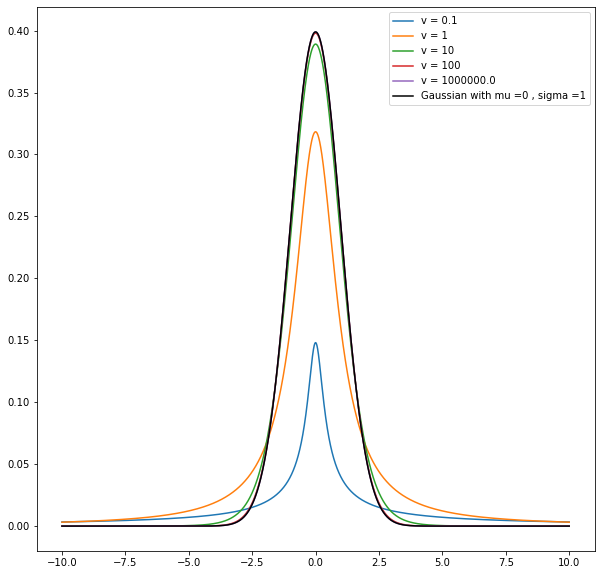
\includegraphics[width=0.8 \linewidth]{P1.png}}
 \end{minipage}
 \end{center}
}
\item~[5 points] Draw the density plots for Beta distributions: Beta(1,1), Beta(5, 5) and Beta (10, 10). Put the three density curves in one figure. What do you observe? Next draw the density plots for Beta(1, 2), Beta(5,6) and Beta(10, 11). Put the three density curves in another figure. What do you observe?
{\red \bf Answer. }{\blackblue  
From Figure 1 (left picture), we can see that Beta distribution ${\rm Beta}(a,a)$ for $a=1$ is just the uniform distribution over $[0,1]$ and then it gets more and more bell shaped concentrated around $x=\frac12$ as $a$ increases. 

Similarly, from Figure 1 (right picture), we observe that that Beta distribution ${\rm Beta}(a,a+1)$ for $a=1$ is a distribution whose density is linearly 
decreasing on $[0,1]$ while it starts to get bell shaped and concentrated around $x=\frac12$ as $a$ increases.	
\begin{figure}[H]
\begin{center}
\begin{minipage}{0.4\textwidth}
     \frame{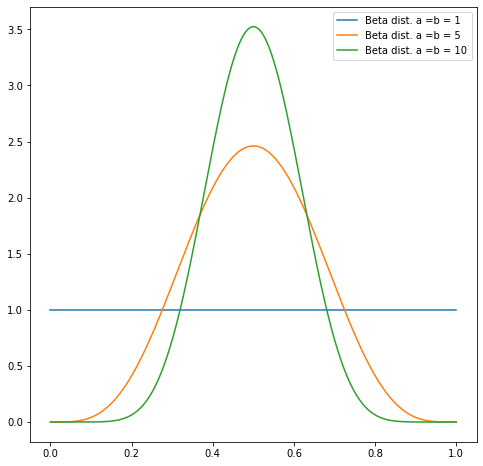
\includegraphics[width=0.85 \linewidth]{P2a.png}}
     \caption{{\footnotesize $\text{Beta}(a,a)$ for  $a\in\{1,5,10\}$}}\label{Fig.2}      
     \end{minipage}
     \begin{minipage}{0.4\textwidth}
     \frame{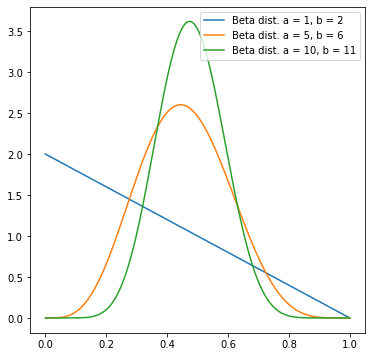
\includegraphics[width=0.85 \linewidth]{P2b.png}}
     \caption{{\footnotesize $\text{Beta}(a,a+1)$ for $a\in\{1,5,10\}$}}\label{Fig.2}
 \end{minipage}
 \end{center}
\end{figure} }
\vspace{-1cm}	
	\item~[10 points] Randomly draw 30 samples from a Gaussian distribution $\N(0, 2)$. Use the 30 samples as your observations to find the maximum likelihood estimation (MLE) for a Gaussian distribution and a student $t$ distribution. For both distributions, please use L-BFGS to optimize the parameters. For student $t$, you need to estimate the degree of the freedom as well. Draw a plot of the estimated the Gaussian distribution density, student $t$ density and the scatter data points. What do you observe, and why? Next, we inject three noises into the data: we append $\{8, 9, 10\}$ to the $30$ samples. Find the MLE for the Gaussian and student $t$ distribution again. Draw the density curves and scatter data points in another figure. What do you observe, and why? 

{\red \bf Answer.}{\blackblue 
	Comparing Figures 3 and 4, we can see that when there is no noisy points added, the MLE estimation for gaussian and student t's models are resulting pretty the same. But, as the noisy points were added, the MLE estimation for gaussian model was more affected by noise rather than the MLE estimation for student t's model.  
\begin{figure}[H]
\begin{center}
\begin{minipage}{0.4\textwidth}
     \frame{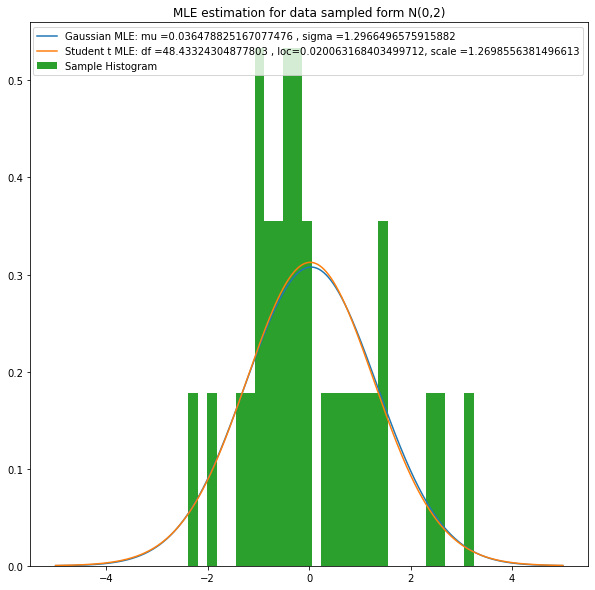
\includegraphics[width=0.95 \linewidth]{P3a.png}}
     \caption{{\footnotesize MLE estimation for $30$ samples fron $\mathcal{N}(0,2)$ }}\label{Fig.2}      
     \end{minipage}
     \begin{minipage}{0.4\textwidth}
     \frame{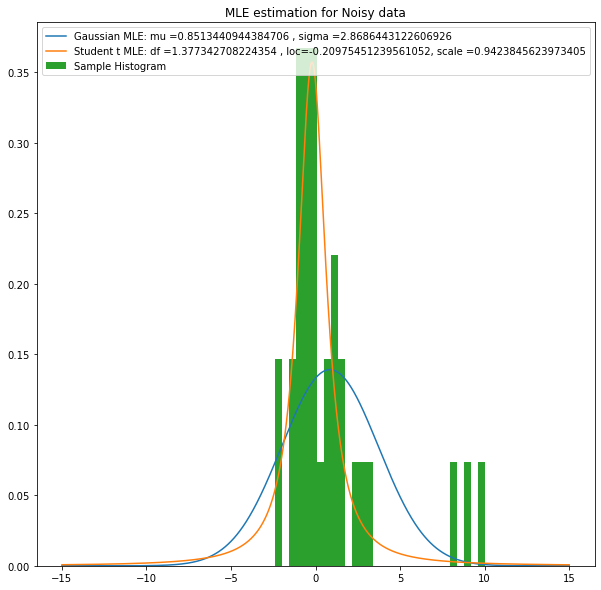
\includegraphics[width=0.95 \linewidth]{P3b.png}}
     \caption{{\footnotesize MLE estimation for noisy samples from $\mathcal{N}(0,2)$}}\label{Fig.2}
 \end{minipage}
 \end{center}
\end{figure}	
}
	

	
\end{enumerate}
\end{document}
%%% Local Variables:
%%% mode: latex
%%% TeX-master: t
%%% End:
